

\chapter{Randbedingungen}

\section{Technische Randbedingungen}

Das verteilte Steuerungssystem unterliegt mehreren festgelegten technischen Rahmenbedingungen, die den Entwicklungs- und Implementierungsspielraum einschränken. Diese Bedingungen sind im Folgenden aufgeführt:

\begin{figure}[h]  
    \centering
    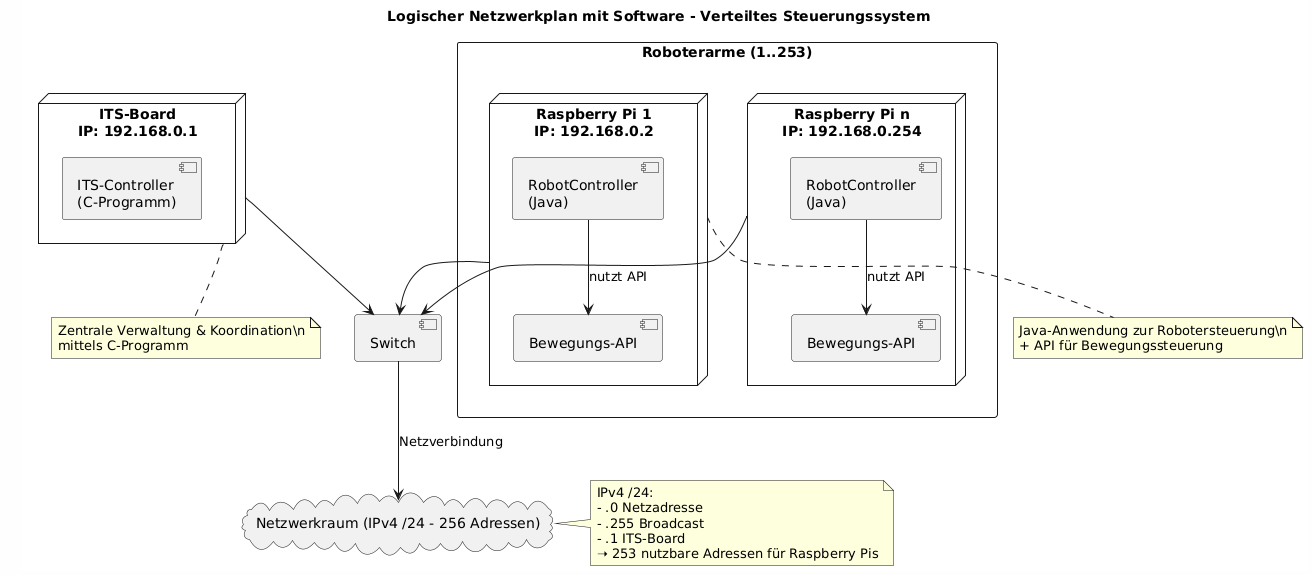
\includegraphics[width=0.8\linewidth]{diagrams/Netzplan.png}
    \caption{Skizze der technischen Randbedingungen}
    \label{fig:Skizze}
\end{figure}



\section{Organisatorische Randbedingungen}
\begin{itemize}

    \item \textbf{Umgebung:}  
    Der Abnahme bereich befindet sich im Raum BT7 R7.65. Die Steuerung und Navigation des Roboters müssen innerhalb der räumlich definierten Grenzen erfolgen. Die dort vorhandene LAN-Infrastruktur kann zur Netzwerkkommunikation verwendet werden.
    \item \textbf{Zeit:} Entwicklungszeitraum beträgt 12 Wochen. 
    \item \textbf{Vorwissen:} Einige Konzepte und Herangehensweisen werden erst im Laufe der 12 Wochen gelernt.
    \item \textbf{Budget:} Es steht kein Budget zur Verfügung.

\end{itemize}

%\section{Konventionen}
